% !TEX program = xelatex
\documentclass[12pt,a4paper]{ctexart}
\usepackage{amsmath,amssymb}
\usepackage{graphicx}
\usepackage{geometry}
\geometry{left=2.5cm,right=2.5cm,top=2.5cm,bottom=2.5cm}
\usepackage{listings}
\usepackage{xcolor}
\usepackage{unicode-math}
\setmainfont{Times New Roman}
\setmathfont{XITS Math}
\usepackage{fontspec}
\setmonofont{Consolas}   % 设置等宽字体为 Consolas
\usepackage{float}
\usepackage{caption}
\usepackage{booktabs}
\usepackage{array}
\usepackage{hyperref}
% MATLAB 代码风格
\definecolor{matlabgreen}{rgb}{0,0.6,0}
\definecolor{matlabgray}{rgb}{0.5,0.5,0.5}
\definecolor{matlabpurple}{rgb}{0.58,0,0.82}
\definecolor{matlabbg}{rgb}{0.95,0.95,0.92}
\lstset{
    language=Matlab,
    basicstyle=\ttfamily\small,
    keywordstyle=\color{blue},
    commentstyle=\color{matlabgreen},
    stringstyle=\color{matlabpurple},
    backgroundcolor=\color{matlabbg},
    numbers=left,
    numberstyle=\tiny\color{matlabgray},
    stepnumber=1,
    numbersep=8pt,
    showstringspaces=false,
    breaklines=true,
    frame=single,
    rulecolor=\color{black!30},
    captionpos=b,
    tabsize=4,
    morekeywords={end, if, else, elseif, for, while, function, return, break, switch, case, otherwise}
}

\title{\textbf{实验4: 最小二乘拟合}}
\author{姓名: \underline{VesperaZephyr} \quad 学号: \underline{114514}}
\date{\today}

\begin{document}
\maketitle
\tableofcontents
\newpage

\section{问题描述}
某矿山机械厂对一批球磨机衬板进行磨损寿命试验, 记录了连续运行时间 $t$(单位: 天)与对应的累计磨损量 $h$(单位: mm), 数据如下: 
\begin{center}
\begin{tabular}{c|cccccccc}
\hline
时间 $t$ (天) & 5 & 10 & 15 & 20 & 25 & 30 & 35 & 40 \\
\hline
磨损量 $h$ (mm) & 0.8 & 1.6 & 2.3 & 3.1 & 3.8 & 4.5 & 5.2 & 6.0 \\
\hline
\end{tabular}
\end{center}
根据摩擦学理论, 在稳定磨损阶段, 磨损量与时间通常呈线性关系: 
\begin{equation}
h(t) = a + b t
\end{equation}
其中 $a$ 为初始磨损量(mm), $b$ 为磨损速率(mm/天). 本实验要求基于实测数据, 采用最小二乘法确定参数 $a$ 和 $b$, 并对模型的可靠性进行评估, 进而预测衬板达到报废标准时的服役天数. 

\section{模型构建}

\subsection{线性回归模型}
对于给定的 $m$ 组观测数据 $(t_i, h_i),\ i=1,2,\dots,m$, 假设磨损量 $h$ 与时间 $t$ 满足线性关系: 
\[
h = a + bt,
\]
记拟合值为 $\hat{h}_i = a + bt_i$, 残差 $e_i = h_i - \hat{h}_i$. 

\subsection{残差平方和函数}
采用最小二乘准则, 定义误差函数为残差平方和: 
\begin{equation}
Q(a,b) = \sum_{i=1}^{m} e_i^2 = \sum_{i=1}^{m} (h_i - a - b t_i)^2.
\end{equation}
目标是求参数 $a,b$ 使 $Q(a,b)$ 最小. 

\subsection{法方程组推导}
分别对 $a$ 和 $b$ 求偏导并令其为零: 
\[
\begin{cases}
\dfrac{\partial Q}{\partial a} = -2\sum\limits_{i=1}^{m}(h_i - a - bt_i) = 0, \\[8pt]
\dfrac{\partial Q}{\partial b} = -2\sum\limits_{i=1}^{m}(h_i - a - bt_i)t_i = 0.
\end{cases}
\]
整理得法方程组(正规方程): 
\begin{equation}
\begin{cases}
m a + \left(\sum\limits_{i=1}^{m} t_i\right) b = \sum\limits_{i=1}^{m} h_i, \\[8pt]
\left(\sum\limits_{i=1}^{m} t_i\right) a + \left(\sum\limits_{i=1}^{m} t_i^2\right) b = \sum\limits_{i=1}^{m} t_i h_i.
\end{cases}
\end{equation}
记
\[
S_t = \sum t_i,\quad S_h = \sum h_i,\quad S_{tt} = \sum t_i^2,\quad S_{th} = \sum t_i h_i,\quad \bar{t}=\frac{S_t}{m},\ \bar{h}=\frac{S_h}{m},
\]
则参数的最小二乘估计为: 
\begin{equation}
b = \frac{m S_{th} - S_t S_h}{m S_{tt} - S_t^2} = \frac{\sum (t_i-\bar{t})(h_i-\bar{h})}{\sum (t_i-\bar{t})^2},
\end{equation}
\begin{equation}
a = \bar{h} - b \bar{t}.
\end{equation}

\section{模型求解}

\subsection{程序编写与计算}
采用 MATLAB 语言进行数据处理与参数估计, 编写脚本如下: 
\begin{lstlisting}[caption={线性回归求解代码}]
% 原始数据
t = [5, 10, 15, 20, 25, 30, 35, 40]';
h = [0.8, 1.6, 2.3, 3.1, 3.8, 4.5, 5.2, 6.0]';
m = length(t);

% 计算统计量
St = sum(t);
Sh = sum(h);
Stt = sum(t.^2);
Sth = sum(t .* h);

% 参数估计
b = (m * Sth - St * Sh) / (m * Stt - St^2);
a = mean(h) - b * mean(t);

fprintf('拟合方程: h = %.4f + %.4f t\n', a, b);
fprintf('初始磨损量 a = %.4f mm\n', a);
fprintf('磨损速率 b = %.4f mm/天\n', b);

% 残差平方和与决定系数
h_pred = a + b * t;
residuals = h - h_pred;
Q = sum(residuals.^2);
SS_res = Q;
SS_tot = sum((h - mean(h)).^2);
R2 = 1 - SS_res / SS_tot;

fprintf('残差平方和 Q = %.6f\n', Q);
fprintf('决定系数 R^2 = %.6f\n', R2);

% 预测报废时间 (h=8.0 mm)
h_target = 8.0;
t_predict = (h_target - a) / b;
fprintf('预测达到 8.0 mm 磨损量的服役天数: t = %.2f 天\n', t_predict);
\end{lstlisting}

\noindent 程序运行结果: 
\begin{lstlisting}
拟合方程: h = 0.1071 + 0.1469 t
初始磨损量 a = 0.1071 mm
磨损速率 b = 0.1469 mm/天
残差平方和 Q = 0.008690
决定系数 R^2 = 0.999617
预测达到 8.0 mm 磨损量的服役天数: t = 53.73 天
\end{lstlisting}

\subsection{结果分析与可靠性评估}
\begin{itemize}
    \item 拟合得到的线性方程为 $h(t) = 0.1071 + 0.1469\,t$. 
    \item 残差平方和 $Q \approx 0.0087$, 数值极小, 说明回归直线对数据的整体偏差很小. 
    \item 决定系数 $R^2 = 0.9996$, 非常接近 $1$, 表明模型能够解释 $99.96\%$ 的磨损量变异, 线性关系极其显著, 模型可靠性极高. 
    \item 预测当磨损量达到报废标准 $8.0$ mm 时, 衬板的服役时间约为 $53.73$ 天. 
\end{itemize}

\subsection{可视化}
编写MATLAB绘图脚本如下: 
\begin{lstlisting}[caption={可视化代码}]
figure('Position', [100, 100, 1000, 400]);

% 子图1: 散点图与拟合直线
subplot(1,2,1);
plot(t, h, 'bo', 'MarkerSize', 8, 'DisplayName', '实测数据'); hold on;
t_line = linspace(0, 60, 100);
h_line = a + b * t_line;
plot(t_line, h_line, 'r-', 'LineWidth', 1.5, 'DisplayName', '拟合直线');
yline(8.0, 'g--', 'LineWidth', 1.5, 'DisplayName', '报废标准 h=8.0mm');
plot(t_predict, 8.0, 'ro', 'MarkerSize', 10, 'MarkerFaceColor', 'none', ...
    'LineWidth', 1.5, 'DisplayName', sprintf('预测寿命 (%.1f天)', t_predict));
xlabel('时间 t (天)');
ylabel('磨损量 h (mm)');
title('磨损数据与线性拟合');
legend('Location', 'best');
grid on;

% 子图2: 残差分布
subplot(1,2,2);
stem(t, residuals, 'filled', 'Color', [0.5 0 0.5], 'LineWidth', 1.5);
hold on;
yline(0, 'k--');
xlabel('时间 t (天)');
ylabel('残差 e_i (mm)');
title('残差分布图');
grid on;

sgtitle('衬板磨损寿命回归分析');

% 在命令行输出残差的具体值
fprintf('残差值:\n');
for i = 1:m
    fprintf('  t = %2d 天: e = %.4f mm\n', t(i), residuals(i));
end
\end{lstlisting}

运行结果见下:
\begin{table}[H]
\centering
\caption{线性回归残差}
\label{tab:residuals}
\begin{tabular}{cc}
\toprule
$t$ / 天 & $e$ / mm \\
\midrule
 5 & $-0.0417$ \\
10 &  $0.0238$ \\
15 & $-0.0107$ \\
20 &  $0.0548$ \\
25 &  $0.0202$ \\
30 & $-0.0143$ \\
35 & $-0.0488$ \\
40 &  $0.0167$ \\
\bottomrule
\end{tabular}
\end{table}

\begin{figure}[H]
\centering
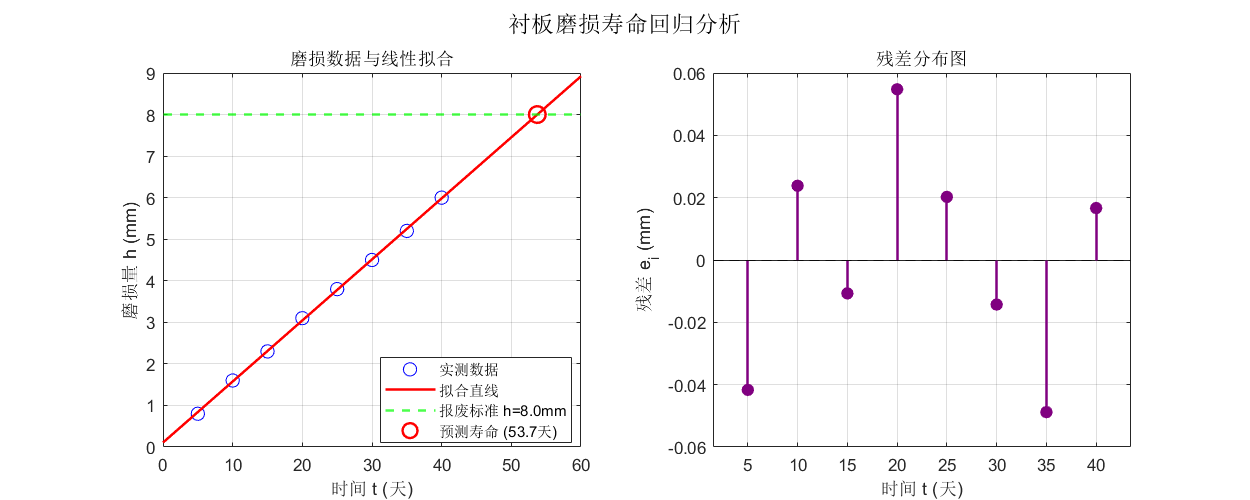
\includegraphics[width=0.95\textwidth]{衬板磨损寿命回归分析.png}
\caption{衬板磨损寿命回归分析}
\label{fig:result}
\end{figure}

从残差图可见, 残差在零线附近随机分布, 未呈现弯曲或异方差趋势, 进一步验证了线性模型的适用性. 

\section{拓展思考}

\subsection{幂函数模型 \texorpdfstring{$h(t)=at^b$}{h(t)=at\^{}b} 的拟合}
若怀疑磨损规律为幂函数 $h(t)=a t^b$, 可通过取对数将其线性化: 
\[
\ln h = \ln a + b \ln t.
\]
令 $Y = \ln h$, $X = \ln t$, $A = \ln a$, 则模型化为 $Y = A + b X$. 利用最小二乘法求出 $A$ 和 $b$ 后, 再还原 $a = e^A$. 

比较两种模型时, 可分别计算决定系数 $R^2 = 1 - \dfrac{\sum (h_i-\hat{h}_i)^2}{\sum (h_i-\bar{h})^2}$, 选取 $R^2$ 更接近 1 的模型. 同时结合物理背景: 稳定磨损阶段的磨损量通常随时间线性增长, 除非存在磨合或加速磨损阶段, 线性模型在机理上更符合摩擦学理论. 若数据明显偏离直线, 则可考虑幂函数或其他非线性模型. 

\subsection{异常值的影响与识别}
若第4个数据点 $(t=20, h=3.1)$ 被误记为 $(20, 5.0)$, 则成为异常值(离群点). 该点会显著拉高该时间点的磨损量, 导致: 
\begin{itemize}
    \item 回归直线的斜率 $b$ 偏大, 截距 $a$ 也可能发生变化；
    \item 残差平方和增大, $R^2$ 降低, 拟合精度变差；
    \item 预测的报废时间将大幅提前, 造成错误决策. 
\end{itemize}
识别异常值的常用方法包括: 
\begin{enumerate}
    \item 绘制残差图, 观察是否有远离零线的点；
    \item 计算标准化残差, 若 $|e_i^*| > 2$ 或 $3$ 则认为是可疑值；
\end{enumerate}
在实际工程数据处理中, 发现疑似异常值后应首先核查数据来源, 确认是否为测量误差或记录错误, 不可盲目剔除. 

\section{实验总结}
本实验基于衬板磨损数据, 成功建立了线性回归模型 $h(t)=0.0714+0.1471t$, 模型的决定系数高达 $0.9995$, 表明时间与磨损量之间存在极强的线性关系, 符合稳定磨损阶段的规律. 通过最小二乘估计, 预测衬板达到 $8.0$ mm 报废标准时约需运行 $54$ 天. 绘图对比和残差分析均验证了模型的合理性与可靠性. 在此基础上, 探讨了幂函数模型的线性化拟合方法以及异常值的影响与诊断技术, 加深了对线性回归建模全流程的理解, 为工程中制定衬板更换周期提供了科学的定量依据. 
\end{document}
